
Análogamente al código, vamos a mostrar la aplicación de los principios descritos en el apartado~\nameref{par:testing} únicamente en los casos más didácticos y relevantes. En proceso de diseño de los tests para el caso de uso~\nameref{subsubsec:CreateTaskUseCase} primero identificamos los factores o variables independientes:

\begin{itemize}
    \item Host
    \item Port
    \item CommunicationMode
    \item ExecutionMode
    \item Steps
\end{itemize}

luego extraemos las clases de equivalencia:

\begin{itemize}
    \item Host: valid/invalid
    \item Port: valid/invalid
    \item CommunicationMode: valid/invalid
    \item ExecutionMode: valid/invalid
    \item Steps: valid/invalid
\end{itemize}

En este caso no aplica el criterio de valores límite. Hay que prestar atención al trabajo de buscar las clases de equivalencia, no es trivial. Por ejemplo, en el caso de steps, que es un array podría haberse pensado que se necesita probar con varios elementos en el array, validos e invalidos, pero no tiene sentido porque la lógica debe contemplar únicamente el caso de uso. Es tarea de la clase Step verificar este tipo de lógicas. Otro ejemplo en el caso de Host o Port que tiene validaciones. podría pensarse que debería ponerse a prueba con varios casos que den invalido, al ser un string libre y que ponga a prueba dicha validación, pero estamos en el caso de uso, eso será responsabilidad del test unitario de Host y Port. para la lógica que nos atañe en este test lo único que importa es qué sucedera en el caso que sea válido o invalido. En un ejemplo tan trivial puede llevar a subestimar el ejercicio de entender el alcance de la prueba y la correcta selección de las clases de equivalencia, pero es de suma importancia.

Con estas clases de equivalencia las posibilidades son $2^5 = 32$. Aplicamos el metodo pairwise de~\nameref{variablesDependendientes} y se reducen a 6 los tests. Los pares posibles son 41. las combinaciones posibles se aprecian en el ~\cref{tab:pairsCreateTaskUseCase} y los pares en el ~\cref{tab:combCreateTaskUseCase}. Los test a implementar finalmente se pueden ver en el ~\cref{tab:createTaskPairWiseTest}

\begin{table}[H]
    \small
    \begin{tabular}{cccccc}
        \textbf{}   & \textbf{host} & \textbf{port} & \textbf{communicationMode} & \textbf{executionMode} & \textbf{sentences} \\
        \textbf{1}  & valid         & valid         & valid                      & valid                  & valid              \\
        \textbf{2}  & valid         & valid         & valid                      & valid                  & invalid            \\
        \textbf{3}  & valid         & valid         & valid                      & invalid                & valid              \\
        \textbf{4}  & valid         & valid         & valid                      & invalid                & invalid            \\
        \textbf{5}  & valid         & valid         & invalid                    & valid                  & valid              \\
        \textbf{6}  & valid         & valid         & invalid                    & valid                  & invalid            \\
        \textbf{7}  & valid         & valid         & invalid                    & invalid                & valid              \\
        \textbf{8}  & valid         & valid         & invalid                    & invalid                & invalid            \\
        \textbf{9}  & valid         & invalid       & valid                      & valid                  & valid              \\
        \textbf{10} & valid         & invalid       & valid                      & valid                  & invalid            \\
        \textbf{11} & valid         & invalid       & valid                      & invalid                & valid              \\
        \textbf{12} & valid         & invalid       & valid                      & invalid                & invalid            \\
        \textbf{13} & valid         & invalid       & invalid                    & valid                  & valid              \\
        \textbf{14} & valid         & invalid       & invalid                    & valid                  & invalid            \\
        \textbf{15} & valid         & invalid       & invalid                    & invalid                & valid              \\
        \textbf{16} & valid         & invalid       & invalid                    & invalid                & invalid            \\
        \textbf{17} & invalid       & valid         & valid                      & valid                  & valid              \\
        \textbf{18} & invalid       & valid         & valid                      & valid                  & invalid            \\
        \textbf{19} & invalid       & valid         & valid                      & invalid                & valid              \\
        \textbf{20} & invalid       & valid         & valid                      & invalid                & invalid            \\
        \textbf{21} & invalid       & valid         & invalid                    & valid                  & valid              \\
        \textbf{22} & invalid       & valid         & invalid                    & valid                  & invalid            \\
        \textbf{23} & invalid       & valid         & invalid                    & invalid                & valid              \\
        \textbf{24} & invalid       & valid         & invalid                    & invalid                & invalid            \\
        \textbf{25} & invalid       & invalid       & valid                      & valid                  & valid              \\
        \textbf{26} & invalid       & invalid       & valid                      & valid                  & invalid            \\
        \textbf{27} & invalid       & invalid       & valid                      & invalid                & valid              \\
        \textbf{28} & invalid       & invalid       & valid                      & invalid                & invalid            \\
        \textbf{29} & invalid       & invalid       & invalid                    & valid                  & valid              \\
        \textbf{30} & invalid       & invalid       & invalid                    & valid                  & invalid            \\
        \textbf{31} & invalid       & invalid       & invalid                    & invalid                & valid              \\
        \textbf{32} & invalid       & invalid       & invalid                    & invalid                & invalid
    \end{tabular}
    \caption{Pares en el diseño de tests para CreateTaskUseCase}\label{tab:pairsCreateTaskUseCase}
\end{table}

\begin{table}[H]
    \small
    \begin{tabular}{llll}
        \textbf{var1}          & \textbf{var2}     & \textbf{value1} & \textbf{value2} \\
        host          & port              & valid           & valid           \\
        host          & port              & valid           & notValid        \\
        host          & port              & notValid        & valid           \\
        host          & port              & notValid        & notValid        \\
        host          & executionMode     & valid           & valid           \\
        host          & executionMode     & valid           & notValid        \\
        host          & executionMode     & notValid        & valid           \\
        host          & executionMode     & notValid        & notValid        \\
        host          & communicationMode & valid           & valid           \\
        host          & communicationMode & valid           & notValid        \\
        host          & communicationMode & notValid        & valid           \\
        host          & communicationMode & notValid        & notValid        \\
        host          & steps             & valid           & valid           \\
        host          & steps             & valid           & notValid        \\
        host          & steps             & notValid        & valid           \\
        host          & steps             & notValid        & notValid        \\
        port          & executionMode     & valid           & valid           \\
        port          & executionMode     & valid           & notValid        \\
        port          & executionMode     & notValid        & valid           \\
        port          & executionMode     & notValid        & notValid        \\
        port          & communicationMode & valid           & valid           \\
        port          & communicationMode & valid           & notValid        \\
        port          & communicationMode & notValid        & valid           \\
        port          & communicationMode & notValid        & notValid        \\
        port          & steps             & valid           & valid           \\
        port          & steps             & valid           & notValid        \\
        port          & steps             & notValid        & valid           \\
        port          & steps             & notValid        & notValid        \\
        executionMode & communicationMode & valid           & valid           \\
        executionMode & communicationMode & valid           & notValid        \\
        executionMode & communicationMode & notValid        & valid           \\
        executionMode & communicationMode & notValid        & notValid        \\
        executionMode          & steps             & valid           & valid           \\
        executionMode          & steps             & valid           & notValid        \\
        executionMode          & steps             & notValid        & valid           \\
        executionMode          & steps             & notValid        & notValid        \\
        communicationMode      & steps             & valid           & valid           \\
        communicationMode      & steps             & valid           & notValid        \\
        communicationMode      & steps             & notValid        & valid           \\
        communicationMode      & steps             & notValid        & notValid
    \end{tabular}
    \caption{Combinaciones en el diseño de tests para CreateTaskUseCase}\label{tab:combCreateTaskUseCase}
\end{table}

\begin{table}[H]
    \small
    \begin{tabular}{rllllll}
        case & host     & port     & ExeMode  & ComMode  & steps    & Expected Result        \\
        1    & valid    & valid    & valid    & valid    & valid    & OK                     \\
        2    & valid    & notValid & notValid & notValid & notValid & PortInvalidError       \\
        3    & notValid & valid    & notValid & valid    & notValid & HostInvalidError       \\
        4    & notValid & notValid & valid    & notValid & valid    & HostInvalidError       \\
        5    & ~valid   & valid    & valid    & notValid & notValid & CommunicationModeError \\
        6    & ~valid   & notValid & notValid & valid    & valid    & PortError
    \end{tabular}
    \caption{Test para CreateTaskUseCase}\label{tab:createTaskPairWiseTest}
\end{table}

En la instanciación de una nueva Task los factores o variables independientes son:

\begin{itemize}
    \item Number of steps
    \item execution Mode
    \item Communication Mode
\end{itemize}

Las clases de equivalencia:

\begin{itemize}
    \item Number of steps: $0, 1, >2$
    \item execution Mode: Automatic, Manual
    \item Communication Mode: Server Stream,Client Stream, Bidirectional y Unary
\end{itemize}

tenemos entonces  $3*2*4 = 24$ posibilidades. Pares obtenemos 27 que aplicando pairwise se reducen a 13 casos. Vemos que la eficiencia en reducción de casos disminuye cuanto menos combinaciones hay. El diseño de los tests queda tal y como se ve en el~\cref{tab:taskTestPairwiseCases}

\begin{table}[H]
    \small
    \begin{tabular}{ccccl}
        \textbf{}   & \textbf{NSteps} & \textbf{ExeMod} & \textbf{ComMode} & \multicolumn{1}{c}{\textbf{Expected Result}}  \\
        \textbf{1}  & 0               & automatic       & serverStream     & NewTaskMustHaveAtLeastOneStepError            \\
        \textbf{2}  & 1               & automatic       & clientStream     & OK                                            \\
        \textbf{3}  & 1               & manual          & bidirectional    & OK                                            \\
        \textbf{4}  & 1               & automatic       & unary            & OK                                            \\
        \textbf{5}  & 1               & manual          & serverStream     & OK                                            \\
        \textbf{6}  & \textgreater{}2 & manual          & unary            & CommunicationModeCanOnlyHaveOneStepError      \\
        \textbf{7}  & \textgreater{}2 & automatic       & serverStream     & CommunicationModeCanOnlyHaveOneStepError      \\
        \textbf{8}  & \textgreater{}2 & manual          & clientStream     & OK                                            \\
        \textbf{9}  & \textgreater{}2 & automatic       & bidirectional    & ManualBidirectionalTaskOnlyCanHave2StepsError \\
        \textbf{10} & 0               & automatic       & clientStream     & TaskMustHaveAtLeastOneStepError               \\
        \textbf{11} & 0               & manual          & bidirectional    & TaskMustHaveAtLeastOneStepError               \\
        \textbf{12} & 0               & automatic       & unary            & TaskMustHaveAtLeastOneStepError               \\
        \textbf{13} & 0               & manual          & serverStream     & TaskMustHaveAtLeastOneStepError
    \end{tabular}
    \caption{Tests para la instanciación de Task}\label{tab:taskTestPairwiseCases}
\end{table}

Ahora vamos a ver cómo la arquitectura protege la calidad del sistema de las implementaciones en proceso de investigación. El looper es el punto más complejo de la aplicación. Está muy ligado a la tecnología gRPC. Extraer la lógica perteneciente al Dominio de la interacción con la infraestructura es algo que no se puede diseñar sin conocimiento previo de la tecnología. En la figura~\cref{fig:testingLooper}, señalado en el segundo recuadro rojo, tenemos el adaptador de comunicación gRPC. Hemos extraido toda la lógica posible a este servicio de dominio, pero dentro de dicho adaptador hay código experimental que puede tener múltiples errores inesperados: no conseguir comunicar con el servicio cliente, timeouts, malas implementaciones de la librería, por ejemplo. Hemos protegido al dominio de todo esto mediante una interfaz que garantiza que ante cualquier error se devuelve siempre un resultado. De esta forma aunque no funcione correctamente la lógica de negocio es clara y concisa, dejando al proceso iterativo ir mejorando la infraestructura. Tengamos en cuenta que hemos extraido de toda la comunicación con el cliente una interfaz útil y única para comunicarnos, una lógica de negocio que entender en pocas lineas de código y explicar su funcionamiento

Se ha de señalar que en el proceso de descubrimiento del lenguaje sabemos que hay un punto débil en el Dominio. Cada una de las gorutines lanzadas pudiera ocurrir que el proceso no consiguiera terminar y se quedara la gorutine en un proceso infinito. Para ello, Golang dispone de una herramienta llamada context que permite gestionar los timeouts de las gorutines evitando que que queden procesos hijos sin control.

\begin{figure}[h]
    \centering
    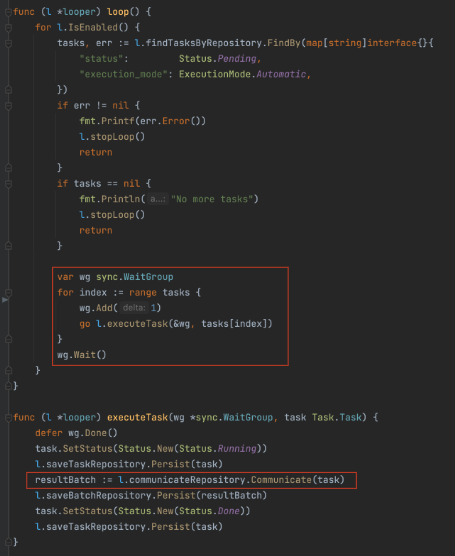
\includegraphics[height=0.5\textheight]{./part/Ejecucion/Seguimiento/Testing/img/Looper}
    \caption{testing looper.go detail}\label{fig:testingLooper}
\end{figure}

Si a esto le hubieramos sumado las lineas de codigo que hay detrás de la interfaz de comunicacion (178) sería ingestionable. Para cuantificar esto vamos a hacer una aproximación al diseño del test necesario para cubrir el adaptador de comunicacion. Se apreciará que en el mismo diseño de los tests queda patente de forma objetiva la debilidad del código. El código completo se encuentra en el repositorio github, en este ejercício didáctico hemos simplificando en pseudocódigo, sería el siguiente:

\begin{verbatim}
connection, err := grpc.Dial()
    serverStream:
        client.CallServerStream(request)
        responseStream.Recv()
    Bidirectional:
        client.CallBidirectional()
        async stream.Recv()
        async stream.Send()
        stream.CloseSend()
    ClientStream:
        client.CallClientStream()
        stream.Send
        stream.CloseAndRecv()
    Unary
        client.CallUnary()
connection.Close()
\end{verbatim}

Hay mucha lógica en un mismo servicio, múltiples responsabilidades y por lo tanto no es un buen diseño. Como se demuestra mejor es intentando diseñar los tests. Para empezar extraer del código las clases de equivalencia y factores no ha sido sencillo. Hay multiples gestiones de errores dispersos por toda su extensión. Esto ocurre en multitud de ocasiones, ya sea debido al tiempo, desconocimiento o mala praxis nos encontramos con códigos de esta magnitud. La arquitectura y todo este proceso lo que hace es protegernos de estas secciones sucias. Los factores serían:

\begin{itemize}
    \item grpc.Dial(): err, connection
    \item client.CallServerStream(request): err,stream
    \item responseStream.Recv(): EOF,err,nil
    \item client.CallBidirectional(): error,stream
    \item stream.Recv(): EOF,err, result
    \item stream.Send(): EOF, nil,err
    \item stream.CloseSend() err,nil
    \item client.CallClientStream(): err, stream
    \item stream.Send: err, nil
    \item stream.CloseAndRecv(): err, nil
    \item client.CallUnary(): err,nil
    \item connection.Close(): err, nil
\end{itemize}

Si no entendieramos bien el concepto de clase de equivalencia podría llevarnos a un mal diseño de los tests y a hacerlo aún más complejo. Aunque hay factores que tiene tres respuestas posibles EOF y nil tienen que ir de la mano, significa que no ha habido error, primero obtienes un nil en el error y luego obtienes un error tipo EOF que significa que todo ha terminado correctamente. y luego tenemos cuando obtenmos un error distinto de EOF, si esto ocurre nos importa cuántas veces haya ocurrido el caso sin error, será error igualmente. Con lo cual las clases de equivalencia serían:

\begin{itemize}
    \item grpc.Dial(): err, connection
    \item client.CallServerStream(): err,stream
    \item responseStream.Recv(): nil\&EOF,err
    \item client.CallBidirectional(): error,stream
    \item stream.Recv(): nil\&EOF,err
    \item stream.Send(): nil\&EOF,err
    \item stream.CloseSend() err,nil
    \item client.CallClientStream(): err, stream
    \item stream.Send: err, nil
    \item stream.CloseAndRecv(): err, nil
    \item client.CallUnary(): err,nil
    \item connection.Close(): err, nil
\end{itemize}

para este caso tendríamos $ 2^{12} = 4096 $ combinaciones posibles que pairwise reduce a 59 tests. aquí se ve la potencia del método. Volviendo posible un testing con ciertas garantías incluso en un código mal diseñado como el que nos ocupa.
